\chapter{Implementation}
\label{impl}
\section{Data collection}
The entire data collection suite is written in JavaScript for Node.js and can 
be found in the \texttt{tinder-gather} directory. The Google Chrome extension 
is also written in JavaScript and the name of its project directory is 
\texttt{tinder-gather-connect}.

\texttt{tinder-gather} is a web application which was made possible using the 
Express.js web application framework. It provides a RESTful HTTP API to manage 
data collection jobs as well as a few debugging pages for viewing face 
detection results.

Profiles and user images found using a modified version of the Tinder.js 
library that implements the Tinder API are stored on disk in the 
\texttt{tinder-gather/gather-images} directory. The metadata for both profiles 
and images is stored in a PostgreSQL database using an ORM library called 
Sequelize, which means it can be easily swapped for an alternative SQL 
database.

Figure \ref{fig:impl:erd_basic} shows the ER diagram for the data collection-
specific part of the database as well as entity \texttt{Detection Job} which 
will be covered in Section \ref{impl:fd}.

The names in parentheses correspond to the actual, case-sensitive table names 
in the PostgreSQL database. 
\begin{figure}[t]
  \centering
  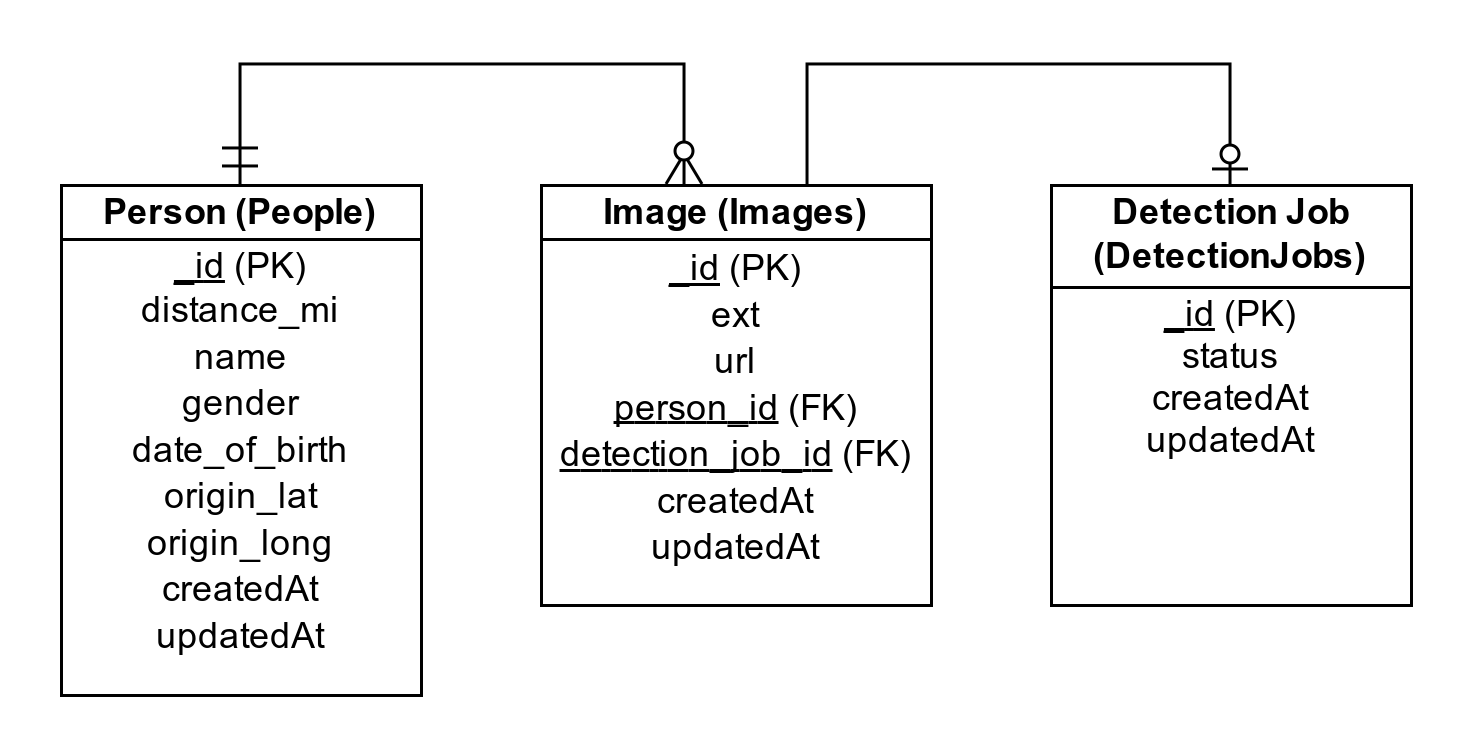
\includegraphics[width=\textwidth]{figures/impl/erd_basic}
  \caption{Entity-relation diagram for tables used by the data collection 
  application \texttt{tinder-gather}. }
  \label{fig:impl:erd_basic}
\end{figure}

\begin{table}[t]
    \begin{center}
        \begin{tabular}{ c  c  c }
            \toprule
            Attribute       & Data type              & Other \\ \toprule
            \multicolumn{3}{c}{Person (People)} \\ \midrule
            \_id           & character(24)            & not null   \\ 
            distance\_mi   & integer                  &            \\ 
            name          & character varying(255)   &            \\ 
            gender        & integer                  &            \\ 
            date\_of\_birth & integer                  &            \\ 
            origin\_lat    & double precision         &            \\ 
            origin\_long   & double precision         &            \\ 

            \midrule
            \multicolumn{3}{c}{Image (Images)} \\ \midrule
            \_id              & character(36)            & not null   \\ 
            ext              & character varying(4)     &            \\ 
            url              & character varying(255)   &            \\ 
            person\_id        & character(24)            &            \\ 
            detection\_job\_id & integer                  &            \\ 

            \midrule
            \multicolumn{3}{c}{Detection Job (DetectionJobs)} \\ \midrule
            \_id      & integer                     & not null, auto-increment \\ 
            status    & enum{started, finished}      &         \\ 

            \midrule
            \multicolumn{3}{c}{Common among all tables} \\ \midrule
            createdAt & timestamp with time zone     & not null  \\ 
            updatedAt & timestamp with time zone     & not null  \\  \bottomrule
        \end{tabular}
    \end{center}
    \caption{Attribute data types of entities introduced in Figure 
    \ref{fig:impl:erd_basic}}
    \label{table:impl:erd_basic_dt}
\end{table}
\subsection{Authentication}
A Google Chrome extension was written in order to obtain an authentication 
token for the Tinder app on Facebook which must be sent with every request to 
the Tinder API. The extension adds a button to the Google Chrome toolbar which 
opens a static web page that sends a request back to the extension to open the 
following URL:
\begin{logs}
https://www.facebook.com/v2.0/dialog/oauth
    ?response_type=token
    &display=popup
    &api_key=464891386855067
    &redirect_uri=fbconnect%3A%2F%2Fsuccess
    &scope=user_about_me%2Cuser_activities%2Cuser_education_history%2Cuser_location%2Cuser_photos%2Cuser_relationship_details%2Cuser_status'
\end{logs}
where \texttt{api\_key} specifies the Tinder application ID on Facebook and 
\texttt{scope} lists the type of information Tinder will gain access to. This 
page asks the user to sign in with their Facebook credentials and, if 
successful, will save a cookie that will be sent along with the next request:

\begin{logs}
POST https://www.facebook.com/v2.0/dialog/oauth/confirm

{
  "app_id: "464891386855067",
  "ttstamp: "2658170904850115701205011500",
  "redirect_uri": "fbconnect://success",
  "return_format": "access_token",
  "from_post": 1,
  "display": "popup",
  "gdp_version": 4,
  "sheet_name": "initial",
  "__CONFIRM__": 1
}
\end{logs}
The response to this will contain an access token that will be used to 
interact with the Tinder API. It can be extracted using 
\begin{logs}
    access_token=([\w_]+)&
\end{logs} 
as a regular expression. It will be referred to as \texttt{<fb\_token>} from 
this point on.

Before we can use it to authenticate with Tinder the Facebook user ID must 
also be obtained by accessing 
\texttt{https://graph.facebook.com/me?access\_token=\textbf{<access\_token>}}.
The response to this request is a JSON object which contains the Facebook user 
ID under the property \texttt{id}, which will be known as 
\texttt{<fb\_user\_id>}.

Now that we have the Facebook user ID and User Access Token it is possible to 
authenticate with Tinder as follows:

\begin{logs}
POST https://api.gotinder.com/auth

{
    "facebook_token": <access_token>, 
    "facebook_id": <fb_user_id>
}
\end{logs}

The response to this request is a JSON object containing Tinder's own 
authentication token and user ID. Tinder's authentication token is saved in 
memory and sent as an HTTP header \texttt{X-Auth-Token} with every request 
after authentication.


\subsection{Updating location}
Updating the location of the user profile is simply a matter of sending the 
new latitude and longitude values via a \texttt{POST} request as follows:
\begin{logs}
POST https://api.gotinder.com/user/ping

{
    "lat": <new_latitude>
    "lon": <new_longitude>
}
\end{logs}
This is performed after authentication with latitude and longitude as 
specified in the data collection job (see \ref{spec:data:jobs}).

The limitation with this method of changing own location is that it is not 
possible to change the location too frequently if the distance between the new 
and the old locations is too large to be travelled in the amount of time 
passed.

\subsection{Fetching profiles and images}
User profiles are internally referred to as \textit{recommendations} by Tinder and 
can be retrieved using the following \texttt{POST} request:
\begin{logs}
POST https://api.gotinder.com/user/recs

{
    "limit": <job_limit>
}
\end{logs}
The \texttt{limit} option refers to the maximum number of users that can be 
fetched at once. The value for \texttt{limit} comes from the corresponding 
data collection job (\ref{spec:data:jobs}).

The JSON response contains a property called \texttt{results} which is an 
array of profiles (\texttt{Array<Profile>}). Every profile contains properties 
as specified in Table \ref{table:profile-properties}.
\begin{table}
    \begin{center}
        \begin{tabular}{| l | c | c |}
            \hline
            Property       & Data type               & Example \\ \hline
            distance\_mi   & integer                 & 2 \\ \hline
            \_id           & char[24]                & 518d666a2a00df0e490000b9 \\ \hline
            birth\_date    & RFC 3339 date and time  & 1986-05-17T00:00:00.000Z \\ \hline
            gender         & integer                 & 1 \\ \hline
            name           & string                  & Elen \\ \hline
            photos         & Array<Photo>            & N/A \\ \hline
        \end{tabular}
    \end{center}
    \caption{Properties of a Tinder profile as retrieved using the API. 
        Properties not used in this project have been stripped out.}
    \label{table:profile-properties}
\end{table}
% "url": "http://images.gotinder.com/518d666a2a00df0e490000b9/fea4f480-7ce0-4143-a310-a03c2b2cdbc6.jpg"
Table \ref{table:photo-properties} shows the relevant properties of profile 
photos.

\begin{table}
    \begin{center}
        \begin{tabular}{| l | c | c |}
            \hline
            Property       & Data type               & Example \\ \hline
            \_id           & UUID                    & fea4f480-7ce0-4143-a310-a03c2b2cdbc6 \\ \hline
            fileName       & string                  & fea4f480-7ce0-4143-a310-a03c2b2cdbc6.jpg \\ \hline
            extension      & string                  & jpg \\ \hline
            url            & URL                     & http://images.gotinder.com/<profile\_id>/<image\_id>.jpg \\ \hline
        \end{tabular}
    \end{center}
    \caption{Properties of a Tinder image as retrieved using the API. 
        Properties not used in this project have been stripped out.}
    \label{table:photo-properties}
\end{table}
The request above is performed every \texttt{<delay>} seconds, the value for 
which is specified as part of a data collection job (see \ref{spec:data:jobs}).


\section{Face and landmark detection}
\label{impl:fd}
The original face detection algorithm introduced by \citep{zhu2012face} was
implemented in MATLAB and was deemed unsuitable to be incorporated into this
project as it would have been difficult to integrate it with other parts of the
system. Luckily, there was an existing implementation of the same algorithm in
C++ by eHarmony \citep{eHphotofeature}. This implementation produced a single
executable which takes a trained model in XML format and a single image as
arguments and labels various landmarks and a bounding box for the face. 

It was modified to read a list of new line character-separated list of image
filenames as standard input so that it could process them in bulk. Instead of
labelling landmarks on the original images it was modified to save detection
results to the central database (PostgreSQL). The database server, credentials
and directory containing the given images are specified in a YAML configuration
file which is passed as the only argument to the modified executable.

\subsection{Face detection job prepare tool}
The \texttt{prepare-detect-worker} script is used to generate the list of image
filenames to process and package the images in a single archive so that face
detection could be done on a remote server.

Generating the list of image filenames to process is done using a Node.js
script executed from inside \texttt{prepare-detect-worker}. It connects to the
central database and fetches image filenames from the \texttt{Images} table
where field \texttt{detection\_job\_id} is the same as the detection job ID
provided as an argument to \texttt{prepare-detect-worker}.

The script then checks if the images actually exist on disk and if not it
downloads the missing images. This is done because the data collection service
may sometimes fail to download an image or it could be invalid. If the image
still cannot be downloaded or contains an error it will be excluded from the
list.

Once the list is generated it is used to create a tar archive using the
standard \texttt{tar} UNIX utility. The filename of the archive would be
\texttt{job-<detection\_job\_id>.tar}.

On the remote face detection server, the \texttt{bulk-detector} script is used
to split the list of images into smaller lists that can be passed to the face
detector executable.

\section{Data analysis and classification}
The entire data analysis and classification stage was implemented in Python
relying on a number of additional packages for image processing, linear
algebra, machine learning and plotting. The dependencies for this project can
be found in the \texttt{requirements.txt} file in the \texttt{data-analysis}
repository. The same file is also used by \texttt{pip}\footnote{Popular Python
package manager.} to download all these dependencies at once.

Unfortunately, not all dependencies could be added to the requirements file as
many of them also depend on certain DEB packages. In order to mitigate these
issues the \texttt{data-analysis} project was modified to run as a Docker
\citep{docker} container so that it could be run on almost any recent Linux
system with minimum configuration.

Before the main \texttt{analysis} script can be used the following commands
must first be executed:
\begin{logs}
    docker build -t="larcher/er-data-analysis" . 
    docker run -i -t larcher/er-data-analysis
\end{logs}
This will start a Docker container and a shell within it from which the main
script \texttt{analysis} can be used. The script uses a configuration file
(\texttt{servers.yaml}) which is used to instruct the data analysis project how
to connect to the PostgreSQL database and where to get the images from. Since
it is an isolated container it will need to download the images from a simple
HTTP server which serves files from \texttt{tinder-gather/gather-images}. This
can be easily done by executing the following command in the
\texttt{tinder-gather/gather-images} directory:
\begin{logs}
    python3 -m http.server 58001
\end{logs}

\subsection{Pre-processing}
As covered in \Cref{spec:analysis:preproc}, the pre-processing stage involved
using the landmark locations put into the PostgreSQL database by the face
detector component to scale, rotate and translate the images so that eye
locations are the same for every image. This was done using numpy for linear
algebra functions to calculate a transformation matrix and OpenCV to perform
affine transformation using this matrix.

\subsection{Feature extraction and classification}
Initially this stage used an implementation of local binary patterns written
specifically for this project, however it was later replaced by a Python
package \citep{facerec} which supports using local binary patterns for feature
extraction and also takes care of classification and model serialisation and
deserialisation.

The support vector machine classifier used in \texttt{facerec} is actually a
wrapper around the \texttt{scikit-learn} implementation of support vector
machines.

The feature extraction method, classifier, classes and cross-validation
parameters are specified in a YAML configuration file which supports running
several experiments at once. 

Experiments can be added to the \texttt{exs} array in the YAML file. For
example, a basic configuration for a single experiment could look like this:
\yamlfile{code/da_simple.yaml}

%%% Local Variables: 
%%% mode: latex
%%% TeX-master: "thesis"
%%% End: 
